% Exercises every construct the package supports, so that a change breaking
% any of them shows up somewhere. Deliberately includes the awkward cases:
% sample lines far too long for their column, a figure, an interactive
% protocol, and a hand-written constraint matrix.
%
% Feature coverage is tracked in the design spec, §9.2.
\documentclass[11pt, a4paper, oneside]{article}
\usepackage[vietnamese, color, standalone]{vnolymp}

\begin{document}

%% ---------------------------------------------------------------------------
%% Named-file I/O, itemised input description, figure, long sample lines
%% ---------------------------------------------------------------------------
\begin{problem}[
  input  = treecut.inp, output = treecut.out,
  time   = 2, memory = 512, points = 100,
  author = {Phan Bình Nguyên Lâm}, origin = {VOI 2026},
]{Chia cây}

Cho một cây gồm $n$ đỉnh, các đỉnh được đánh số từ $1$ đến $n$. Đỉnh thứ $i$
có giá trị $a_i$.

\textbf{Yêu cầu:} Hãy tìm cách xoá cạnh sao cho tổng giá trị các thành phần
liên thông là lớn nhất.

\InputFile
\begin{itemize}
  \item Dòng thứ nhất chứa số nguyên $n$.
  \item Dòng thứ hai chứa $n$ số nguyên $a_1, a_2, \dots, a_n$.
  \item Mỗi dòng trong $n - 1$ dòng tiếp theo chứa hai số nguyên $u_i$, $v_i$
        mô tả một cạnh của cây.
\end{itemize}

\OutputFile
Một số nguyên duy nhất là giá trị lớn nhất có thể đạt được.

\Constraints
$1 \le n \le 3 \cdot 10^5$ và $1 \le a_i \le 10^9$.

\begin{subtasks}
  \subtask{30}{$n \le 20$}
  \subtask{30}{$n \le 2000$, mọi đỉnh có bậc không quá $2$}
  \subtask{40}{Không có ràng buộc gì thêm}
\end{subtasks}

\Examples
% The second sample has lines far wider than the column, which is what the
% line-wrapping in vnolymp-example.def exists for. The old template overflowed
% the margin here without warning.
\begin{example}
\exmpfile{ex1.in}{ex1.out}%
\exmpfile{ex2.in}{ex2.out}%
\end{example}

\Note
Hình dưới minh hoạ ví dụ thứ nhất. Nét đứt là cạnh bị xoá.

\begin{center}
  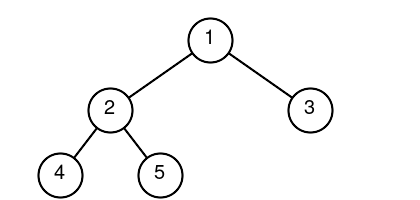
\includegraphics[width=0.45\linewidth]{tree.png}

  Cây trong ví dụ thứ nhất
\end{center}

\end{problem}

%% ---------------------------------------------------------------------------
%% Interactive protocol, inline \texttt literals, hand-written matrix
%% ---------------------------------------------------------------------------
\begin{problem}[
  input = stdin, output = stdout,
  time  = 1, memory = 256, points = 50,
]{Đoán số}

Đây là một bài toán tương tác. Hệ thống chọn một số nguyên bí mật $x$ và bạn
phải tìm ra nó.

\Interaction
Mỗi lượt, bạn in ra một truy vấn dạng \texttt{? y} rồi xuống dòng. Hệ thống
trả lời bằng một trong ba ký tự: \texttt{<}, \texttt{=} hoặc \texttt{>}. Khi
đã biết đáp án, hãy in ra \texttt{! x} và kết thúc chương trình.

\Constraints
$1 \le x \le 10^9$. Số truy vấn không vượt quá $30$.

\Scoring
Điểm được chia theo số truy vấn tối đa mà chương trình sử dụng.

% No dedicated API for a constraint matrix -- by decision, spec §5.2. A matrix
% is a plain tabular the author writes and styles.
\begin{center}
  \begin{tabular}{c c c}
    \hline
    Số truy vấn & $x$ & Điểm \\
    \hline
    $\le 30$ & $\le 10^9$ & $50$ \\
    $\le 60$ & $\le 10^9$ & $25$ \\
    \hline
  \end{tabular}
\end{center}

\Note
Không có ví dụ cho bài toán tương tác.

\end{problem}

\end{document}
